\documentclass[thesis.tex]{subfiles}
\begin{document}

\chapter{Prerequisites}\label{chap:preq}
\todo{single, multi-station?, distance computation?}
\todo{magnitude computation and magnitude scales}
\todo{azimuth and single/multistation}
\todo{Station Codes}
\todo{distance detection up to which point}
\todo{epicentral and hypocentral distance, depth (on an image)}
\todo{magnitudenberechnung klassisch}
\todo{Machine learning intro}
\todo{motivierender Satz}
\todo{Ein Gedanke pro Satz}
\todo{uncertainties in the Model weiter nach hinten}
\todo{dropout erklären}
\todo{peak displacement Bild}
\todo{acceleration, displacement}
\todo{sensitivity}
\section{Earthquake Physics}\label{section:geophysikalische_grundlagen}
\subsection{The Earthquake Event}
An earthquake are caused by movements within the earth crust. These might result from earth plates moving under or against each other or artificial causes like mining works. After building up a lot of stress against friction, rock fractures along a fault line while the other tectonic layers can slip past each other. The fault line can even be visible on the surface. \\
The point where the fracturing starts is called hypocenter, while the epicenter is this point's projection onto the surface as seen in figure \ref{fig:hypocenter}. The breakage can extend to other points along the fault line as well as cause more ruptures. 
\begin{figure*}[h!]
	\centering
	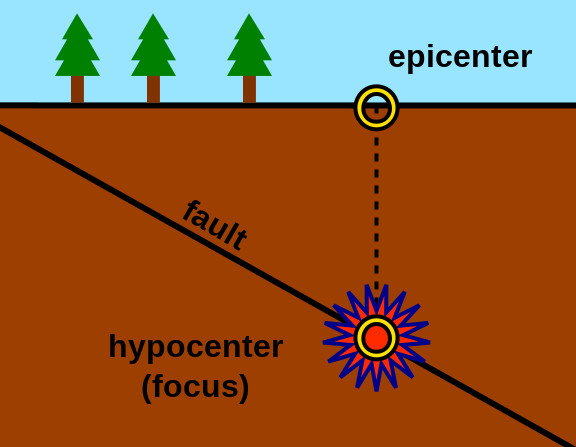
\includegraphics[width=0.6\linewidth]{Prerequisites/Epicenter_Diagram.jpg}
	\caption{Hypocenter and Epicenter}
	\label{fig:hypocenter}
\end{figure*}
\subsection{Seismic Waves} \todo{S waves are dangerous too}
The energy, which is emitted as the fracturing occurs, travels through the earth crust as seismic waves. We denote different types of waves, which travel at different velocities. Soil and material type (air, liquid or solid) also affect wave arrival times. Waves also reflect on certain materials, creating many sub-types of waves to arrive.\\
The first wave to arrive at a site is the p-wave or primary/pressure wave. The propagating waves moves the material back and forth and is therefore also known as a compressional wave. \\
S-waves, second or shear waves move the material in a right angle to the movement direction. Contrary to p-waves, s-waves cannot move through liquid and are slightly slower than p-waves. Figure \ref{fig:speedwaves} shows this relationship.
\begin{figure*}[h!]
	\centering
	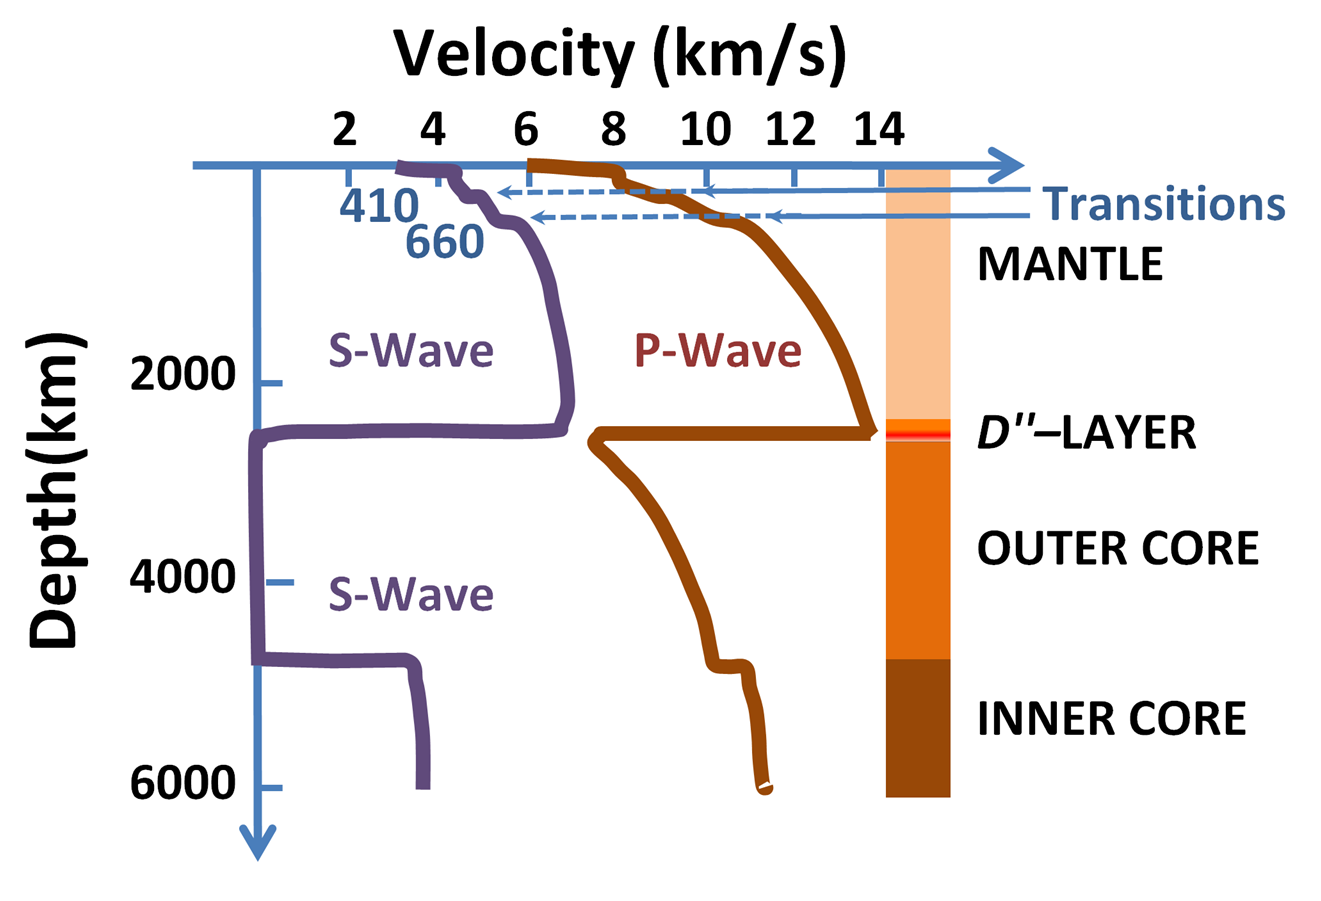
\includegraphics[width=0.6\linewidth]{../pictures/Prerequisites/Speeds_of_seismic_waves.PNG}
	\caption{Velocity of S and p Wave}
	\label{fig:speedwaves}
\end{figure*}
S-Wave and P-Waves are often denoted as body waves. Surface waves arrive even later and are the most damaging ones. Two important waves are Rayleigh and Love waves. Rayleigh waves cause the surface to "ripple", they move the ground up and down while Love waves cause horizontal shearing.
We can see all mentioned types of waves in figure \ref{fig:waves}.¸
\begin{figure*}[h!]
	\centering
	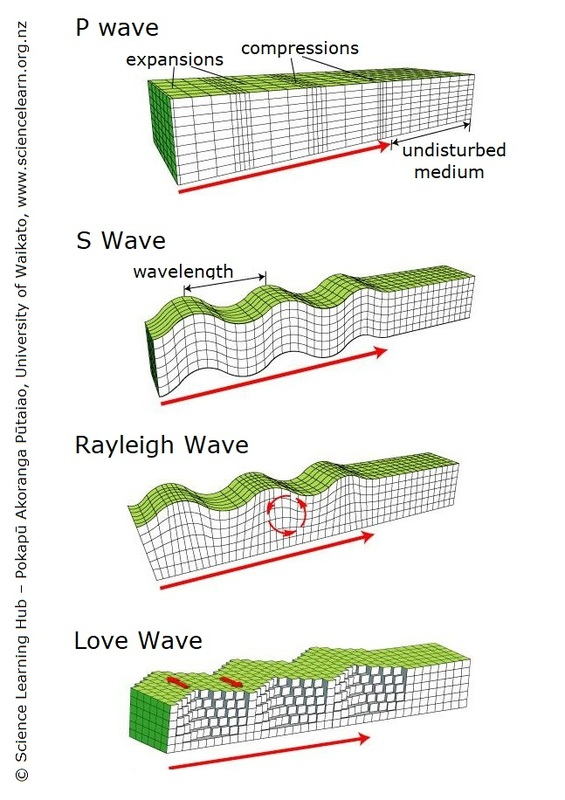
\includegraphics[width=0.6\linewidth]{../pictures/Prerequisites/waves.jpg}
	\caption{Overview of seismic waves}
	\label{fig:waves}
\end{figure*}
\section{Recording an Earthquake}
\subsection{Seismic Data}
The seismic waves which arrive on a site can be recorded by a seismometer, which is the instrument recording ground motion as displacement, velocity or acceleration. A seismograph is the system build around the seismometer. Seismograms show the measured motions as a 1D signal for the three motion orthogonal axes, namely north-south, east-west and ground-up. The recordings depend on the sensitivity of the sensors, but also on earthquake and location. For further reading see \citet{IntroEarthquakes}, page 398. An example for a recording of one axis at an earthquake arrival can be seen in figure \ref{fig:seismogram}. The change from noise to P-Wave to S-Wave arrival is clearly visible in the example. 
\subsection{Networks}
Multiple seismometers might be organized in a network, where stations are linked together virtually or physically and their data can be processed nearly simultaneously. Network goals are often earthquake prediction with the according depth and distance, but network size, sensor type and network range can be drastically different depending on the type and magnitude of earthquake which must be detected. As the emitted waves get weaker depending on distance and soil type good coverage is crucial to get realistic predictions. This is especially important for location computation, as we need three or more sensors on the corners of a preferably equilateral triangle to get a precise location with the circle method. More information on the organisation of sensor networks can be found in \cite{Havskov2016}.
\subsection{Early Warning}
\begin{figure*}[h!]
	\centering
	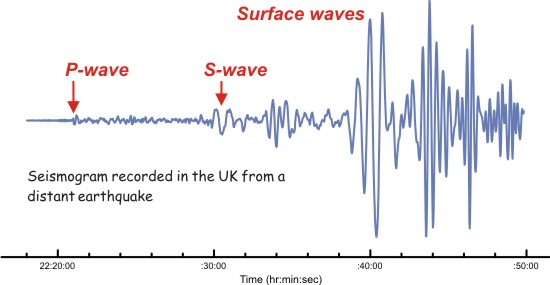
\includegraphics[width=0.6\linewidth]{../pictures/Prerequisites/dia_seismogram.jpg}
	\caption{One axis recording of a seismograph}
	\label{fig:seismogram}
\end{figure*}
\section{Differences between regression and classification}
\subsection{Typical networks and techniques}
\section{Estimation Representation} 
 It is in important to keep in mind, that we do not take into account the uncertainty of our magnitude model and the representation of an earthquake with just ground motion sensors is itself a simplification.
\subsection{Types of uncertainty}
We divide between epistemic and aleatoric uncertainty.
\begin{itemize}
	\item Epistemic uncertainty is our model uncertainty. The model can be unsure about certain parts of our dataset, because it has seen too few data points, but it can also be lacking the design to wholly learn and understand the dataset. The model can also be unsure, if we are unsure about the model's parameters for prediction or if we have multiple models to choose from when predicting. 
	\\
	Epistemic uncertainty can be reduced by adding more training examples and choosing a good model architecture.
	\item Aleatoric uncertainty is uncertainty engrained in the data. This includes instrument noise and (over-)simplification of data information. We further divide between homoscedatic and heteroscedatic aleatoric noise. While homoscedatic uncertainty stays the same for all data point examples, as it would be with a constant sensor-offset noise, heteroscedatic uncertainty can be different for each input sample and is much harder to track and.
\end{itemize}
\subsection{Uncertainties in our model}
There are a few key points in the way our dataset is build which contribute to aleatoric uncertainty. While seismometers are extremely precise instruments, they are not completely free from sensor noise. We remove the sensor response in preprocessing, but they are still physical instruments, which cannot guarantee total precision, although it is more than enough for our model. 
\\
Even more, our learning goals, distance and magnitude are itself hard to determine. The distance to an earthquake has to be assumed from the emitted waves recorded by multiple seismometers and relies on certain simplifications of earthquake physics. As this is the same for the magnitude, the magnitude itself is a physical concept, that tries to capture the strength of an earthquake, but uses a simplified representation of the energy the earthquake emits, which again is only computed on the basis of our recorded data.\\
Epistemic uncertainty is far easier to detect. As also seen in /ref{dataset} our data is not equally distributed and we are lacking examples for higher magnitudes and (naturally, as small earthquakes cannot be detected by remote sensors) higher distances. \\
As distance and magnitude are measurements of our sensor data, the model uncertainty also changes while the signal goes in and out, as earthquake waves arrive and depart. We do expect that, because both magnitude and distance are linked to the wavelength and amplitude of certain emitted waves.
\subsection{Implementation}
A very basic technique is taking the softmax output of a classification network as an uncertainty measure. While this is a good rule-of-thumb, most larger networks are overconfident in their predictions, meaning their accuracy is in general lower than the certainty that is suggested by the softmax output. \cite{guo2017calibration} propose a few methods for improvement. \\
For Bayesian neural networks instead of a single value a gaussian distribution is placed over the weights. Techniques similar to "Bayes by Backprop" \cite{blundell2015weight} allow learning the weight distributions with an algorithm very similar to standard backpropagation. When predicting an example, the weights are sampled from the distribution every time, giving an uncertainty measure for this example after a reasonable number of runs.\\
In contrast to Bayesian neural networks, which require a change of loss functions and learning routines, "Monte Carlo Dropout" does not need this. Instead of just using dropout during training, \cite{gal2016dropout} apply dropout also when predicting examples and generate an uncertainty measure by aggregating the (all slightly different) outputs.\\
An even simpler method, that can be used for regression networks, is not learning a single valued output, but the mean and standard deviation of a gaussian distribution by changing the loss function and the last layer of the network. The mean can then be used as a output prediction, while the standard deviation gives an uncertainty. 



\subfilebib % Makes bibliography available when compiling as subfile
\end{document}